\chapter{Patternidentifikation}
Der nächste Schritt auf dem Weg zur Lokalisierung der \QRCodes ist das Identifizieren der \fps. Dafür wird die durch \OpenCV bereitgestellte \texttt{findContours} Methode verwendet. Sie basiert auf dem Algorithmus von Suzuki und wird eingesetzt, um Konturen im Binärbild zu erkennen.
\inputCPP[label={lst:findcontours}][][Aufruf der \texttt{findContours} Methode]{code/findContours.cpp}
%Listing \ref{lst:findcontours} zeigt den Aufruf um alle Konturen des übergebenen Bildes zu erhalten.

\section{Vorgehensweise des Algorithmus von Suzuki} \label{suzuki}
Iteriere über das Binärbild. Für jeden Pixel $p_{i,j}$ überprüfe ob folgende Bedingungen wahr sind:
\begin{description}
	\item[outer border] Der Farbton des Vorgängers $p_{i,j-1}$ unterscheidet sich vom aktuell betrachteten Pixel $p_{i,j}$. \\Bsp.: $p_{i,j} = 1$ und $p_{i,j-1} = 0$ dann ist $p_{i,j}$ ein Startpunkt eines \emph{outer border}.
	\item[hole border] Sei $x > 1$ ein beliebiger Abstand und es gelte $p_{i,j-x} =\ldots = p_{i,j-1}= 1$ und $p_{i,j} = 0$, dann ist $p_{i,j}$ ein Startpunkt eines \emph{hole border}.
	\\Bsp.: Für $x=2: p_{i,j} = 1$ und $p_{i,j-1} = 0$ und $p_{i,j-2} = 0$ dann ist $p_{i,j}$ ein Startpunkt eines \emph{hole border}.
\end{description}
Sind beide Bedingungen erfüllt, ist der Pixel $p_{i,j}$ ein Anfangspunkt einer neuen Kontur. Diese Kontur muss eindeutig identifizierbar sein, daher wird sie mit einer \emph{KonturID} versehen. Der Vorteil dieses Algorithmus ist, dass so eine Hierarchie der Konturen aufgebaut wird. Dazu muss die \emph{parent}-Kontur für die neue Kontur gesetzt werden. Während der Iteration des Bildes wird immer die äußere Kontur zwischengespeichert. Diese ist entweder eine \emph{parent}-Kontur oder eine Kontur die, die neue Kontur und die \emph{parent}-Kontur teilt. Wenn alle Werte gesetzt sind, wird die Kontur durch sukzessives Hinzunehmen von Pixeln entlang der Kante erzeugt. Das heißt es wird eine Kantenverfolgung durchgeführt. Nach jeder Kontur Erzeugung springt der Algorithmus zurück und führt die Iteration fort. Der Algorithmus terminiert bei Erreichen der rechten unteren Ecke.

Das Original Paper \cite{journals/cvgip/SuzukiA85} beschreibt ausführlich das Vorgehen anhand von Beispielen und Pseudocode.

\section{Filtern der Konturen}
Nachdem die Konturen erkannt wurden, werden Sie mithilfe der durch \texttt{findContours} erstellten Hierarchie gefiltert. Dabei werden Konturen verworfen, die mindestens eine dieser Bedingung erfüllen:
\begin{enumerate}
	\item Die Kontur ist zu klein oder zu groß.
	\item Die Kontur hat keine \emph{parent}-Kontur.
	\item Die Kontur hat Nachbarkonturen.
	\item Die Kontur hat eine \emph{child}-Kontur.
\end{enumerate}
Für jede nicht verworfene Kontur wird ihre zugehörige \emph{parent}-Kontur betrachtet. Für diese muss die Bedingungen $1$ und $3$ gelten.
Zuletzt wird von dieser Kontur noch einmal die nächste \emph{parent}-Kontur betrachtet. Für diese muss wieder Bedingung $1$ zutreffen und außerdem muss diese Kontur eine Trapezoide Form aufweisen.
% Könnte schöner sein.
Um die Trapezoide Form zu überprüfen wird dazu die Form der Kontur mit der \texttt{approxPolyDP} Methode approximiert. Wenn diese aus genau vier Punkten besteht, wird sie als Trapezoid anerkannt.

Falls nicht mindestens drei \fps lokalisiert wurden, wird das nächste Verfahren für die Bildbinarisierung ausgeführt und die Suche beginnt von vorne. Wurden alle Verfahren durchgeführt ohne das ausreichend \fps gefunden wurden, wird angenommen das kein \QRCode im Bild zu finden ist und der Prozess wird beendet.

\section{Kanten Approximation}
Nachdem mehrere Kandidaten von \fps gefunden wurden, wird als nächstes die äußerste Kontur dieser Kandidaten verwendet, um deren Kanten zu approximieren. Zuvor wurden mit \OpenCV und Suzukis Algorithmus \ref{suzuki} alle Konturen \texttt{CV\_CHAIN\_APPROX\_NONE} im Bild lokalisiert, weswegen jede Kontur jetzt eine zusammenhängende Kette von Punkten darstellt. Für jede Kontur sollen mithilfe dieser Punktmenge die vier äußeren Kanten des \fps approximiert werden. Dazu werden die Konturen in vier Segmente aufgeteilt.

\begin{figure}[h]
\centering
\begin{subfigure}[t]{0.48\textwidth}
\centering
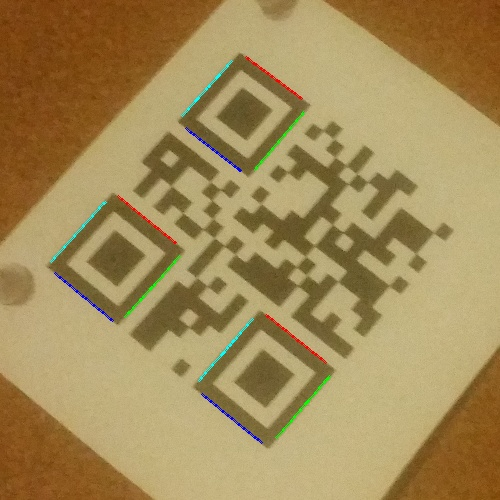
\includegraphics[scale=0.25]{images/qrcode-adler-wand_4___SEGMENTS___.jpg}
\caption{Segmentierung}
\end{subfigure}%
\begin{subfigure}[t]{0.48\textwidth}
\centering
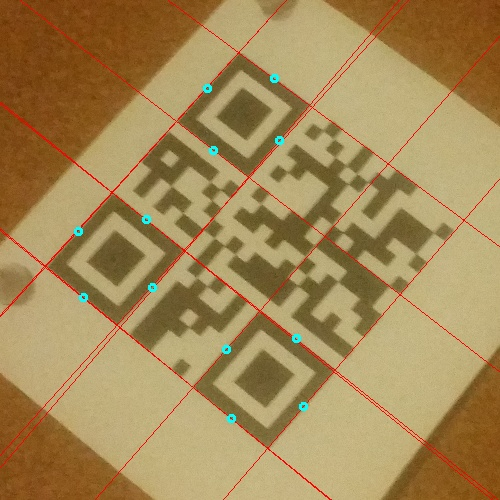
\includegraphics[scale=0.25]{images/qrcode-adler-wand_5___LINES___.jpg}
\caption{Geraden Approximation}
\label{fig:lines}
\end{subfigure}
\caption{Aufteilen der einzelnen Konturen in Segmente und Approximation der Kanten durch Geraden.}
\end{figure}

Es müssen zunächst die Schnittpunkte gefunden werden, an denen die Kontur geteilt werden soll. Dazu werden die bereits zuvor berechneten Punkte, die durch Approximation der Trapezoiden Form der äußersten Kontur gefunden wurden, verwendet. Diese liegen jedoch im Regelfall nicht exakt auf den Ecken der \fps. Außerdem kann schlechte Bildqualität zu Abrundungen oder verschobenen Ecken führen. Um bessere Kanten Approximationen zu erhalten, werden jeweils 10\% aller Punkte am Anfang und Ende jedes Segments verworfen. Diese Segmente werden dann genutzt, um mit der \texttt{fitLine}-Methode die Kanten zu approximieren.

Die \texttt{fitLine}-Methode beruht auf dem Prinzip von \emph{M-Estimators} und verwendet als Minimierungsfunktion den, in \OpenCV durch \texttt{CV\_DIST\_FAIR} definierten, Ausdruck. Die approximierten Geraden werden durch einen Stützvektor und Richtungsvektor beschrieben. Eine wichtige Eigenschaft der Stützvektoren ist, dass Sie sich innerhalb der konvexen Hülle aller Punkte befinden, welche zur Approximation verwendet wurden.
\\\\
Am Ende der Identifikation aller Möglichen \fps sind somit folgende Informationen bekannt:
\begin{itemize}
	\item Mindestens drei \fps
	\item Eine Kontur pro \fp
	\item Vier Segmente pro \fp
	\item Vier Kantengeraden pro \fp
\end{itemize}